\documentclass{article}
\usepackage[utf8]{inputenc}
\usepackage{tabularx}
\usepackage{graphicx}
\usepackage{hyperref}
\usepackage{amsmath}
\usepackage{amssymb}
\usepackage{soul}

\title{ChaLearn Face Anti-spoofing Attack Detection Challenge fact sheets}

\begin{document}

\maketitle

\section{Team details}

\begin{itemize}
\item Team name

VisionLabs

\item Team leader name

Parkin, Aleksandr

\item Team contacts

Address: Vijzelstraat 20, 4th Floor,\\
1017 HK, Amsterdam,\\
the Netherlands\\
Email: a.parkin@visionlabs.ai

\item Rest of the team members

Parkin, Aleksandr (corresponding author)\\
Grinchuk, Oleg


\item Team website URL

\url{https://visionlabs.ai}

\item Affiliation

VisionLabs

\end{itemize}

\section{Contribution details}

\begin{itemize}
\item Title of the contribution

HardTune: Ensembling and Fine-tuning Face Recognition Networks for Multi-Modal Face Anti-spoofing

\item Validation/Final score (if any)

\begin{tabular}{l*{4}{c}}	
             & ACER & tpr@fpr=10e-2 & tpr@fpr=10e-3 & tpr@fpr=10e-4 \\
\hline
Validation   & 0.0000 & 1.0000 & 1.0000 & 1.0000 \\
Test         & 0.0008 & 0.9999 & 0.9996 & 0.9988 \\
\end{tabular}


\item General method description

Our method uses a modified network architecture in [1].
As shown in Figure~\ref{fig:architecture}, the RGB, Depth and IR inputs are processed by separate streams followed by the concatenation and fully-connected layers.
Differently from [1] we use aggregation blocks (Agg res2, ...) to aggregate outputs from multiple layers of the network.
We pre-train network weights on four different tasks for face recognition and gender recognition. 
We then fine-tune these networks separately on the training set of the CASIA-SURF face anti-spoofing dataset.
To increase the robustness to various attacks, we ensemble networks trained on three training folds and with two initial seeds. 
Results of our models evaluated separately and in combination are illustrated in Table~\ref{tab:ensemble}.

%we conbine networks fine-tuned trained with 
%with an addition of aggregating layers from different block levels. For the stability of the solution on testset, which differs from the train by method of attack, we used an ensemble of 4 models, which were pretrained on different datasets, with different architectures and training methods. Each model, mentioned earlier, is an ensemble of 6 networks trained on three folds and with two different random seeds.

\item References

%\begin{thebibliography}{2}
%\bibitem{casia-surf}
[1] Shifeng Zhang, Xiaobo Wang, Ajian Liu, Chenxu Zhao, Jun Wan, Sergio Escalera, Hailin Shi, Zezheng Wang, Stan Z. Li, "CASIA-SURF: A Dataset and Benchmark for Large-scale Multi-modal Face Anti-spoofing", arXiv, 2018. \\

[2] Dong Yi, Zhen Lei, Shengcai Liao, Stan Z. Li, "Learning Face Representation from Scratch", arXiv, 2014. \\

[3] Zhenxing Niu, Mo Zhou, Le Wang, Xinbo Gao, Gang Hua, "Ordinal Regression With Multiple Output CNN for Age Estimation", The IEEE Conference on Computer Vision and Pattern Recognition (CVPR), 2016, pp. 4920-4928 \\

[4] Yandong Guo, Lei Zhang, Yuxiao Hu, Xiaodong He, Jianfeng Gao, "MS-Celeb-1M: Challenge of Recognizing One Million Celebrities in the Real World", 2016

%\end{thebibliography}

\item Representative image / diagram of the method

See Figure~\ref{fig:architecture}.
\begin{figure}
\centering
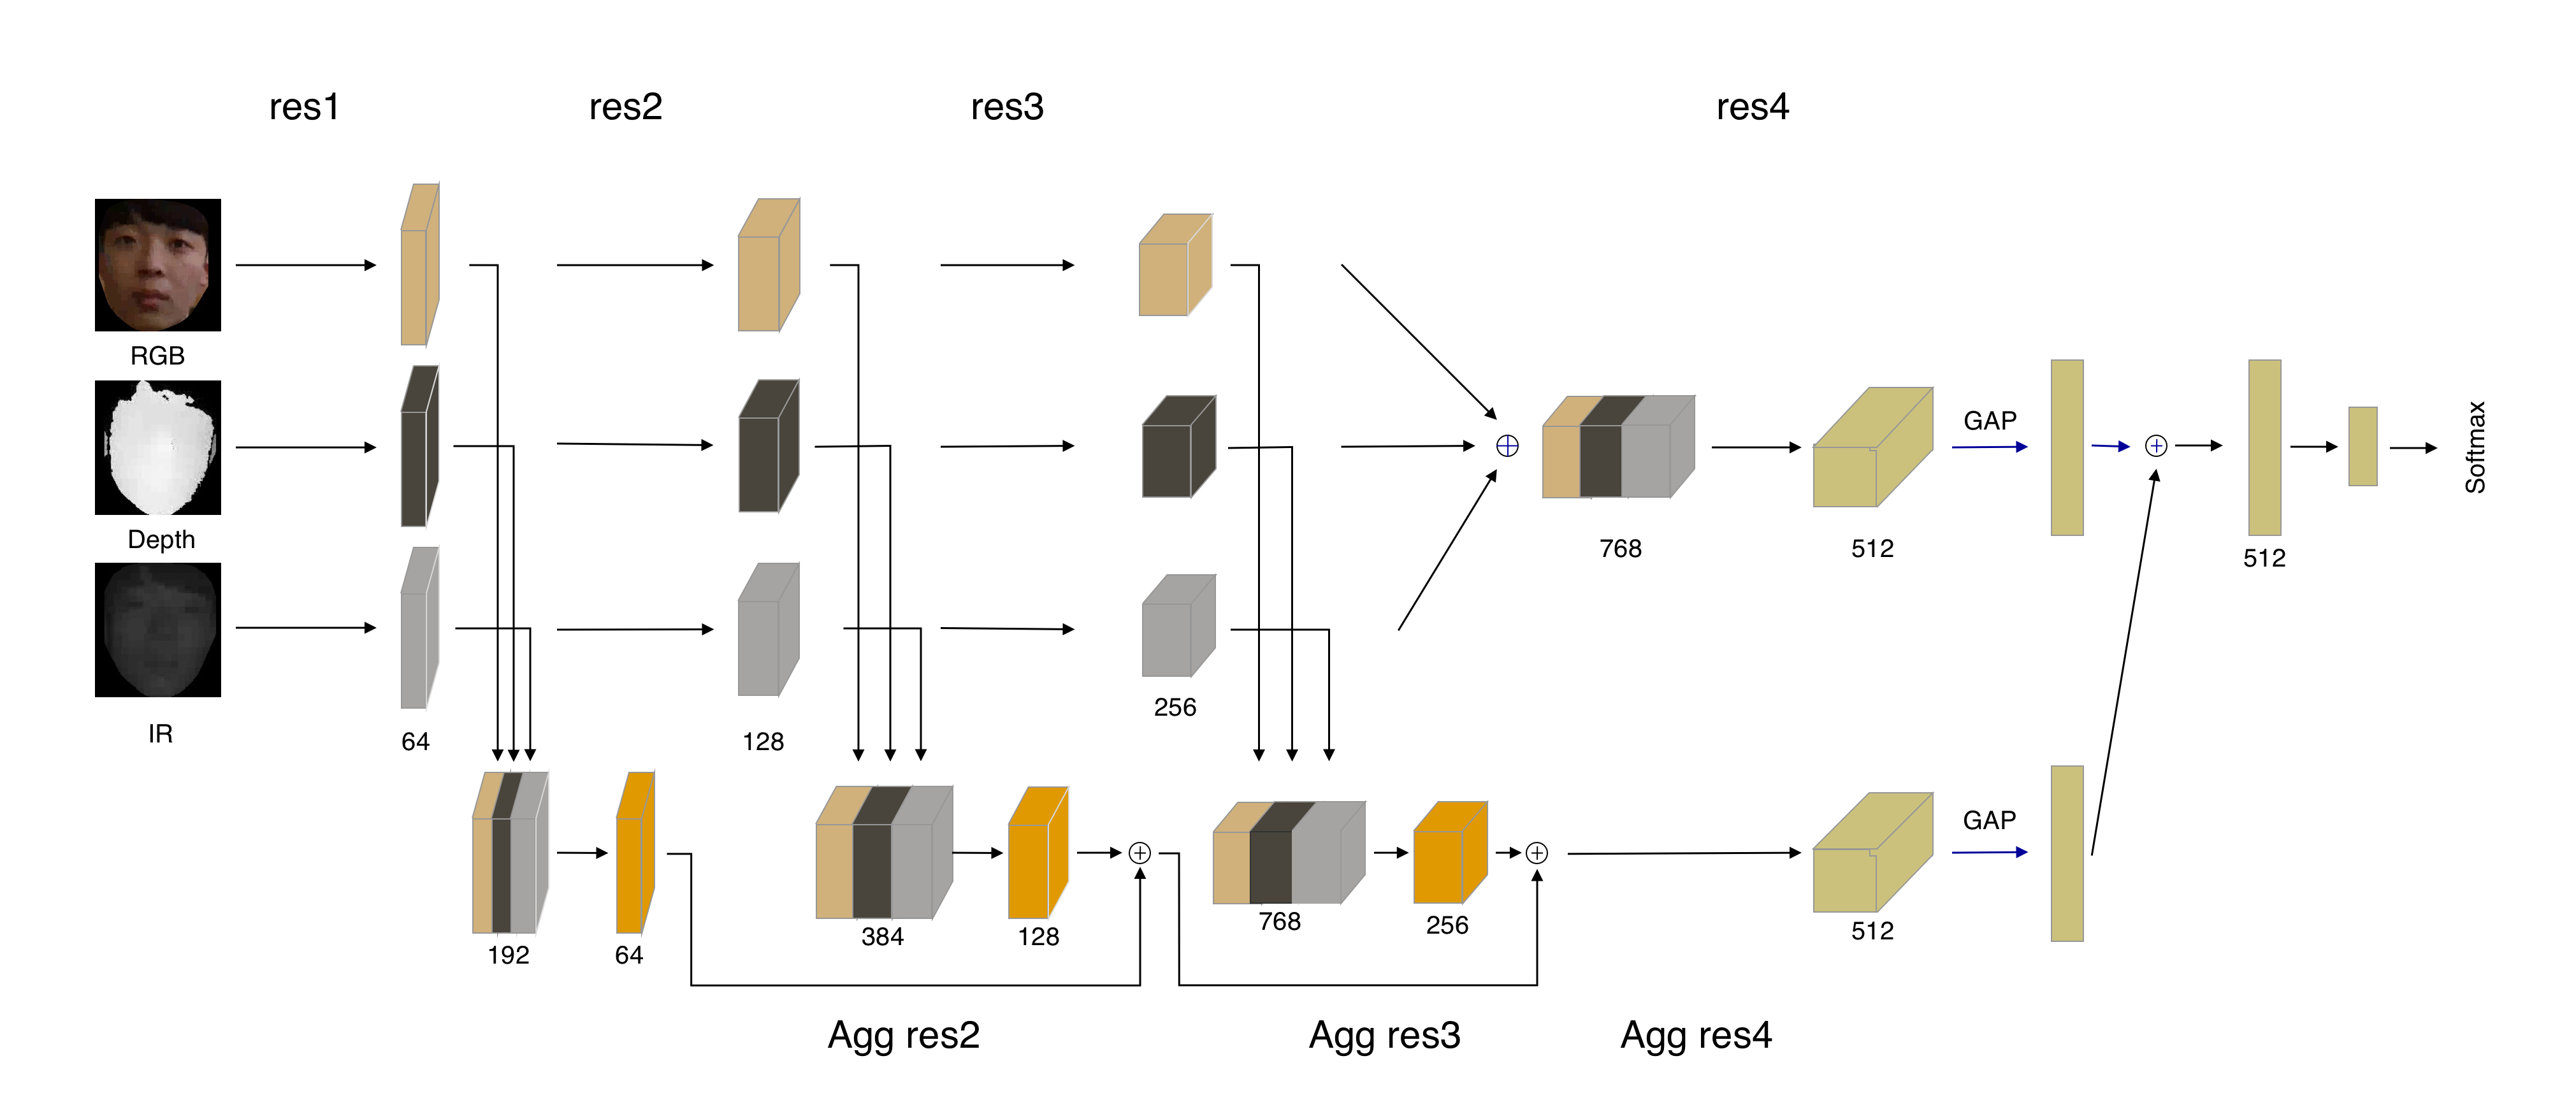
\includegraphics[width=12cm]{figures/net.jpg}
\caption{Deep layer aggregation architecture}
\label{fig:architecture}
\end{figure}


\item Describe data preprocessing techniques applied (if any)

The input image of each modality and its horizontal flip was resized to $125 \times $125 pixels and cropped to $112 \times $112 pixels around the center.

\end{itemize}

\section{Face Anti-spoofing Analysis}

\subsection{Features / Data representation}
%Describe features used or data representation model FOR face anti-spoofing detection (if any)

We use neural networks pre-trained on face and gender recognition tasks as a basis for our submission.

\subsection{Dimensionality reduction}
%Dimensionality reduction technique applied FOR face anti-spoofing detection  (if any)

\subsection{Fusing methods}
%Feature fusing methods, i.e. multi-modality feature fusion, others (if any)


\subsection{Learning strategy}
%Learning strategy applied FOR face anti-spoofing (OR/AND SPOTTING) STAGE (if any)

To increase robustness to unknown attacks, we split the training set into three folds according to different attacks present in the training subset. 
The outputs of three networks were ensembled by averaging to produce results on the final Validation and Test sets.
%For getting stable results on new attack examples training data was splitted on three folds by attack type, two out of three were used for training. The results of the three models were ensembled by averaging.

\medskip
\noindent
We use several learning strategies to train our models:
%For training models we used several different learning rate decay strategies:
\begin{enumerate}
	\item StepLR. Decay learning rate by 0.5 every 15 epochs.
	\item CosineLR. Set learning rate by cosine annealing schedule with the period of 50 epochs
\end{enumerate}

\subsection{Other techniques}
%Other technique/strategy used not included in previous items FOR Face anti-spoofing (if any)

\subsection{Method complexity}
%Method complexity FOR face anti-spoofing
Our final model is an ensemble of 24 networks trained on three folds, using two initial seeds and pre-trained on four face and gender recognition tasks.

\subsection{Data Fusion Strategies}
%List data fusion strategies (how different feature descriptions are combined) for learning the model / network: RGB, depth, ir. (if any)

We fuse information from different modality streams by aggregating feature maps after each ResNet block and concatenates streams after res3 block, as show in Figure~\ref{fig:architecture}. Some of our models also use Squeeze and Excitation module after the res3 block.

\subsection{Global Method Description}

We opted to use an ensemble of various models to get a stable result on the test. The models were added to the ensemble in a greedy manner if they did not decrease the performance on the validation set. Results of our individual models and their combinations are presented in Table~\ref{tab:ensemble}. We provide below descriptions for our individual models.

\begin{table}
\caption{Results on the Validation and Test sets of the challenge. "Seeds" indicates the use of two different initial seeds. See text for the description of different NN models.}
%NN1a replaced NN1 because it showed better results outside the ensemble

% NN1 = exp1
% NN1a = exp1_2stage
% NN2 = exp2
% NN3 = exp3b
% NN4 = exp3c
\begin{center}
\begin{tabular}{cccccc|cc}
& & & & & & Val & Test \\
NN1 & NN1a & NN2 & NN3 & NN4 & Seeds & \footnotesize{tpr@fpr=10e-4} & \footnotesize{tpr@fpr=10e-4}\\
\hline 
\checkmark & & & & & & 0.9943 & -\\
& \checkmark & & & & & 0.9987 & -\\
& & \checkmark & & & & 0.9870 & -\\
& & & \checkmark & & & 0.9963 & -\\
& & & & \checkmark & & 0.9933 & -\\
\checkmark & & \checkmark & & & & 0.9963 & -\\
\checkmark & & \checkmark & \checkmark & & & 0.9983 & -\\
\checkmark & & \checkmark & \checkmark & & \checkmark & 0.9997 & -\\
\checkmark & & \checkmark & \checkmark & \checkmark & \checkmark & 1.0000 & -\\
& \checkmark & \checkmark & \checkmark & \checkmark & \checkmark & \textbf{1.0000} & \textbf{0.9988}\\ \hline
\end{tabular}
\end{center}
\label{tab:ensemble}
\end{table}

\begin{description}
\item[NN1] resnet-34. Pretrain description: facial recognition training on Casia-WebFace[2] with SphereFace loss. Antispoofing training: cosine LR strategy
\item[NN2] resnet-34. Pretrain description: gender recognition training on AFAD-Lite[3], cosine lr strategy. Antispoofing training: cosine LR strategy
\item[NN3] resnet-50. Pretrain description: facial recognition training on MSCeleb-1m with ArcFace loss, cosine LR strategy. Antispoofing training: cosine LR strategy
\item[NN4] resnet-50. Pretrain description: facial recognition training on private asian dataset with ArcFace loss. Antispoofing training: cosine LR strategy
\item[NN1a] resnet-34. Pretrain description: facial recognition training on Casia-WebFace[2] with SphereFace loss. Antispoofing training: step LR strategy, last epoch is trained with weak augmentation
\end{description}

\begin{itemize}
\item Which pre-trained or external methods have been used (for any stage, if any)

Models pre-trained on face recognition tasks have shown best results on the validation. We therefore use the pre-trained ResNet-34 on Casia-WebFace~[2] from adversarial attacks on black box face recognition challenge (\url{https://competitions.codalab.org/competitions/19090}), ResNet-50 trained on MSCeleb-1M~[4] and private asian dataset from public Jian Zhao repository (\url{https://github.com/ZhaoJ9014/face.evoLVe.PyTorch}).

\item Which additional data has been used in addition to the provided ChaLearn training and validation data (at any stage, if any)

We use no additional data specifically dedicated to the anti-spoofing task.
We have trained ResNet-34 for the age recognition task on the AFAD-Lite~[3] dataset to create a pre-trained model.

\item Qualitative advantages of the proposed solution
\item Results of the comparison to other approaches (if any)


\item Novelty degree of the solution and if is has been previously published
\end{itemize}

\section{Other details}

\begin{itemize}
\item Language and implementation details (including platform, memory, parallelization requirements)

We use python with the PyTorch deep learning framework

\item Human effort required for implementation, training and validation?
\item Training/testing expended time?

Training one model takes about three hours on a 4 1080ti GPU. The inference on 1000 images takes about 8 seconds.

\item General comments and impressions of the challenge? what do you expect from a new face anti-spoofing challenge?

The CASIA-SURF dataset is well-prepared and has well-defined train/test splits for the comparison of defence methods against spoofing attacks. 
Meanwhile, we have noticed poor quality of some Depth images. We believe better results could be obtained if Depth input would be saved in the original format.

%Unfortunately, a lot of information was lost during the preprocessing of the depth stream, because instead of saving the distance between face and camera in mm, only the depth map visualization was used.

\end{itemize}

\end{document}
